\chapter{Generalizing the Approach to Arbitrary Combinational Circuits}\label{ch:generalize}
The abstraction approach presented in the previous chapter is
directly applicable only when the word-size of the operands 
of the given circuit are the same, $k$ bits in size. 
In this case, the circuit computes a function over $\F^n_{2^k} \rightarrow \Fkk$, 
where $n$ is the number of word-level inputs,
and the abstraction is thus analyzed over $\Fkk$. 
When the input and output sizes vary, the analysis must be performed 
over an overarching field.
This chapter shows how to suitably modify the approach for
abstracting word-level representations of circuits with varying input and output sizes.

As an application of this generalization, design and verification methodologies 
for composite field multipliers over $\Fkk$ 
are also explored.
These designs decompose the field $\Fkk$ to $\F_{(2^m)^n}$, where 
$k=m\cdot n$. 
Internally, the circuit is then composed of an $n$-interconnection of 
$m$-bit multipliers and adders over $\F_{2^m}$.
This chapter describes how this hierarchy can be exploited by the abstraction
approach.

\section{Circuits with Varying Input and Output Sizes}
When the word size of the inputs and output of the circuits vary, the 
functionality of the circuit must be analyzed over an encompassing composite field. 
Given a circuit with a word-level input $A$ and word-level output $Z$,
let $t$ be the bit size of the $A$ and $u$ be the bit size of $Z$.
Input $A$ can be represented as an element over the field $\F_{2^{t}}$; likewise,
$Z$ is an element of $\F_{2^u}$.
Thus, this circuit computes some function $f: \F_{2^t} \rightarrow \F_{2^u}$.
If $t \neq u$, there is no guarantee that $A$ can be represented over $\F_{2^u}$
and or conversely $Z$ over $\F_{2^t}$. Thus, the analysis must be performed over some 
$\Fkk$ such that $\F_{2^t} \subset \Fkk$ and $\F_{2^u} \subset \Fkk$. 
That is, the function is mapped to a larger field $\Fkk \rightarrow \Fkk$.
The smallest such field $\Fkk$ is constructed where $k = LCM(t,u)$. 

Given the primitive polynomial $P(x)$ of degree $k$, let $\alpha$ be the primitive 
element of $\Fkk$, i.e. $P(\alpha)=0$.
Let $\beta$ be some primitive
element of $\F_{2^t}$. Then the polynomial $f_A$ is denoted 
\begin{equation}
f_A: a_0+a_1\beta+\dots+a_{t-1}\beta^{t-1}+A 
\end{equation}
Since the analysis is over $\Fkk$, $\beta$ must be mapped
directly to $\alpha$. Here, a generalized result from \cite{cf:2003} gives the relation.
%applying Equation \label{eqn:relation} gives the relation.

\begin{equation}
\beta=\alpha^{(2^k-1)/(2^t-1)} \label{eqn:betaToAlpha}
\end{equation}

All powers of $\beta$ in $f_A$ are replaced by their representation in $\alpha$.
Similarly, let $\gamma$ be the primitive element of $\F_{2^u}$, such that
\begin{equation}
f_Z: z_0+z_1\gamma+\dots+z_{u-1}\gamma^{u-1}+Z
\end{equation}
A mapping from $\gamma$ to $\alpha$ is found in the same way and applied to $f_Z$.
All polynomials in the ideal $J$ now have coefficients in $\Fkk$. The polynomials in 
$J_0$ derived from $A$ and from $Z$ are modified to reflect their corresponding fields:
\begin{eqnarray}
A^{2^t}+A=0 & & Z^{2^u}+Z=0
\end{eqnarray}
Now the reduction procedure $f_Z\xrightarrow{F-{f_z},F_0}_+ r$ is 
computed normally over $\Fkk$. 

%Some changes still need to be made to
%functionally map each $\{a_0,\dots,a_{t-1}\}$ to $A$ over $\Fkk$. This is 
%accomplished by first setting up the bit-level to word-level mapping over $\F_{2^t}$ using
%the same approach described in Chapter \ref{ch:improv}. That is, construct the matrix
%\mathbf{M}, which is composed of variable $A$ and coefficients in $\beta$.
%\begin{equation}
%\mathbf{M} = \begin{bmatrix}
%1      &   \beta          & \beta^2           & \dots & \beta^{t-1}\\
%1      &   \beta^2        & \beta^{4}        & \dots & \beta^{(t-1)*2}\\
%1      &   \beta^4        & \beta^{8}        & \dots & \beta^{(t-1)*4}\\
%\vdots & \vdots           & \vdots        & \cdot     & \vdots \\
%1      &   \beta^{2^{t-1}}   & \beta^{2*2^{t-1}} & \dots & \beta^{(t-1)*2^{t-1}}
%\end{bmatrix}
%\end{equation}
%Then,
%map each $\beta$ coefficient in $\mathbf{M}$ to $\alpha$ using 
%Equation \ref{eqn:betaToAlpha}. Since $\beta$ is a primitive element of $\F_{2^t}$,
%each $\{\beta,\beta^2,\dots\beta^{2^{t-1}}\}$ is a distinct element. It follows that,
%once mapped to $\alpha$, each element stays distinct since $\alpha$ is a primitive 
%element of a larger field. Thus, $\mathbf{|M|}\neq 0$, Cramer's rule can be applied, and
%the rest of the approach proceeds as before
%to derive polynomials the $f_{a_0},\dots,f_{a_{t-1}}\}$ over $\Fkk$.
%\begin{eqnarray}
%&f_{a_0} : a_0 + & \nonumber \\
%&\vdots& \nonumber \\
%&f_{a_{k-1}} : a_{k-1} + \Func_{a_{k-1}}(A)& \nonumber
%\end{eqnarray}

Some changes still need to be made to
functionally map each $\{a_0,\dots,a_{t-1}\}$ to $A$ over $\Fkk$. 
This is accomplished by first computing the bit-level to word-level mapping over 
$\F_{2^t}$ using the same approach described in Chapter \ref{ch:improv}, which will provide
the polynomials $f_{a_0},\dots,f_{a_t}$ with coefficients in $\beta$. Then, map each $\beta$ 
coefficient in $F_a = \{f_{a_0},\dots,f_{a_t}\}$ to $\alpha$ using Eqn.(\ref{eqn:betaToAlpha}). 
Polynomials of $F_a$ are now in $\Fkk$ and
the final substitution 
$r\xrightarrow{F_a+J_0}_+r_w$ is computed as normal. 

This allows the word-level abstraction of any combinational circuit with one
word-level input of any size and one word-level output. In the case of multiple
word-level inputs, let $k$ be the $LCM$ of all the bit-sizes of the inputs and
outputs. Then the abstraction proceeds as normal.

\begin{Example}
\begin{figure}[!hbt]
\centerline{
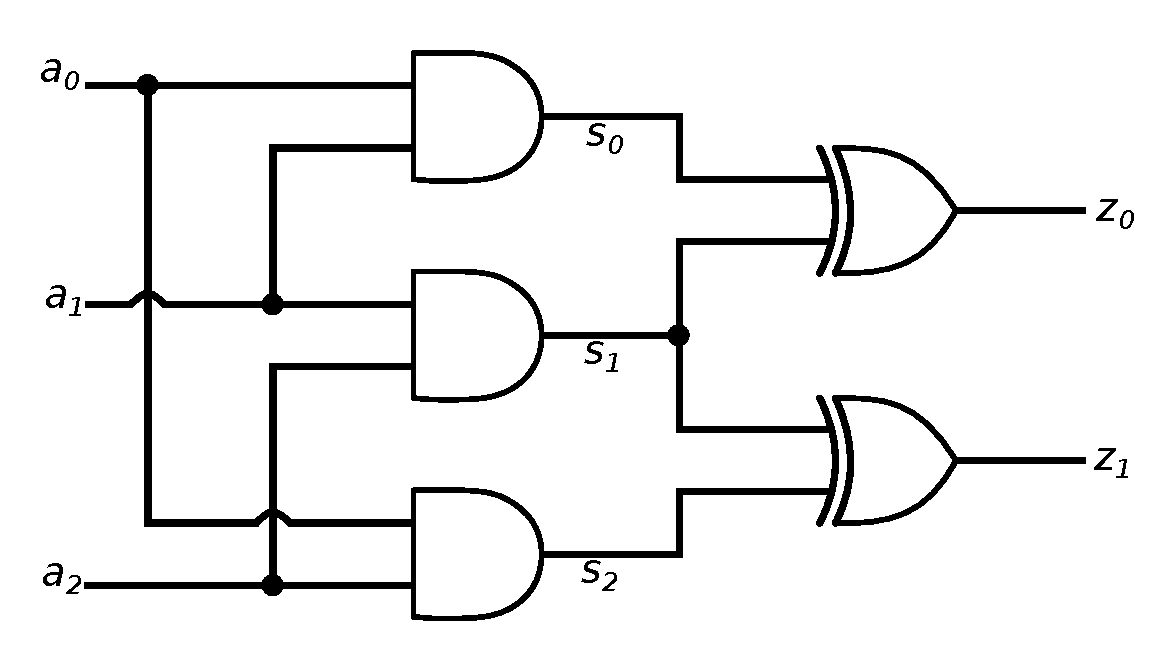
\includegraphics[scale=0.4]{./figures/3to2.eps}
}
\caption{ Circuit with varying word sizes.}
\label{fig:3to2}
\end{figure}
{\it 
Consider the circuit shown in Fig. \ref{fig:3to2}. The input, $A$, is 3 bits 
wide while the output, $Z$ is 2 bits. Thus, $A\in {\mathbb{F}}_{2^3}$ and 
$Z \in {\mathbb{F}}_{2^2}$. Let $\beta$ be the primitive element of 
${\mathbb{F}}_{2^3}$ and $\gamma$ be the primitive element of 
${\mathbb{F}}_{2^2}$, i.e. $A=a_0+a_1\beta+a_2\beta^2$ and $Z=z_0+z_1\gamma$.
Thus, the circuit computes the function ${\mathbb{F}}_{2^3}\rightarrow{\mathbb{F}}_{2^2}$. Since $LCM(2,3)=6$, then $\F_{2^2} \subset \F_{2^6}$ and $\F_{2^3} \subset
\F_{2^6}$. So this function mapped to $\F_{2^6} \rightarrow \F_{2^6}$.
Choose $P(X)=X^6+X+1$ as the irreducible
polynomial to construct $\F_{2^6}$, where $P(\alpha)=0$. Then $\beta$ and
$\gamma$ in can be represented in terms of $\alpha$:
\begin{eqnarray}
\beta=\alpha^{(2^6-1)/(2^3-1)}=\alpha^9 \nonumber \\
\gamma=\alpha^{(2^6-1)/(2^2-1)}=\alpha^{21} 
\end{eqnarray}
So the word-level polynomials are:
\begin{eqnarray}
&&f_A: a_0+a_1\alpha^9+a_2\alpha^{18}+A \nonumber \\
&&f_Z: z_0+z_1\alpha^{21}+Z 
\end{eqnarray}
The rest of the polynomials in $F$ are derived from the circuit:
\begin{eqnarray}
f_1: z_0+s_0+s_1 & f_2: z_1+s_1+s_2 & f_3: s_0+a_0\cdot a_1 \nonumber \\
f_4: s_1+a_1\cdot a_2 & f_5: s_2+a_0\cdot a_2 &
\end{eqnarray}
where the RATO ordering is:
\begin{equation}
z_0 > z_1 > s_0 > s_1 > s_2 > a_0 > a_1 > a_2 > Z > A
\end{equation}
$F_0$ is defined as before, except with a change to the polynomials derived from word-level 
variables $A$ and $Z$:
\begin{eqnarray}
f_6: z_0^2+z_0 & f_7: z_1^2+z_1 & f_8: s_0^2+s_0 \nonumber \\
f_9: s_1^2+s_1 & f_{10}: s_2^2+s_2 & f_{11}: a_0^2+a_0 \nonumber \\
f_{12}: a_1^2+a_2 & f_{13}: a_2^2+a_2 & f_{14}: Z^4+Z \nonumber \\
f_{15}: A^8+A & & 
\end{eqnarray}

Computing $f_Z\xrightarrow{F-{f_z},F_0}_+ r$ gives:
\begin{eqnarray}
r&=& (\alpha^2+\alpha)\cdot a_1\cdot a_2+a_1\cdot A+(\alpha^4+\alpha^3)\cdot a_1 \nonumber \\
&&+(\alpha^5+\alpha^4+\alpha^3+\alpha+1)\cdot a_2\cdot A+(\alpha^5+\alpha^4+\alpha^2+\alpha)\cdot a_2+Z
\end{eqnarray}

This result must be further reduced by $f_{a_1}: a_1 + \Func_{a_1}(A)$ and $f_{a_2}: a_2 + \Func-{a_2}(A)$. 
First, find $\mathbf{M}$ in terms of $\beta$ as derived from $A=a_0+a_1\beta+a_2\beta^2$.
Then map it to $\alpha$.  

\begin{eqnarray}
\mathbf{M}=
\begin{bmatrix}
1      &   \beta   & \beta^2  \\
1      &   \beta^2 & \beta^4  \\
1      &   \beta^4 & \beta^8
\end{bmatrix} & 
\mathbf{M_1}=
\begin{bmatrix}
1      &   A   & \beta^2  \\
1      &   A^2 & \beta^4  \\
1      &   A^4 & \beta^8
\end{bmatrix} &
\mathbf{M_2}=
\begin{bmatrix}
1      &   \beta   & A  \\
1      &   \beta^2 & A^2  \\
1      &   \beta^4 & A^4
\end{bmatrix}
\end{eqnarray}

Computing the determinants in $f_{a_1}: a_1 + |\mathbf{M_1}|$ and $f_{a_2}: a_2 + |\mathbf{M_2}|$ gives:
\begin{eqnarray}
f_{a_1}: a_1+A^4\cdot (\beta^4+\beta^2)+A^2\cdot (\beta^8+\beta^2)+A\cdot (\beta^8+\beta^4) \nonumber \\
f_{a_2}: a_2+A^4\cdot (\beta^2+\beta)+A^2\cdot (\beta^4+\beta)+A\cdot (\beta^4+\beta^2)
\end{eqnarray}
Replacing all $\beta$ in $f_{a_1}$ and $f_{a_2}$ with $\alpha^9$ gives their proper form over $\F_{2^6}$.
\begin{eqnarray}
f_{a_1}: a_1+A^4\cdot(\alpha^4+\alpha^3+1)+A^2\cdot(\alpha^4+\alpha^2+\alpha+1)+A\cdot(\alpha^3+\alpha^2+\alpha) \nonumber \\
f_{a_2}: a_2+A^4\cdot(\alpha^4+\alpha^2+\alpha+1)+A^2\cdot(\alpha^3+\alpha^2+\alpha)+A\cdot(\alpha^4+\alpha^3+1)
\end{eqnarray}

Finally, computing the reduction $r\xrightarrow{f_{a_1},f_{a_2},F_0}_+ r_w$ gives the word-level polynomial
abstraction of the circuit.
%Applying the abstraction approach, the word-level polynomial $Z+\F(A)$ found is

\begin{eqnarray}
r_w:&&Z+A^6(\alpha^2+\alpha)+A^5(\alpha^4+\alpha^3+\alpha)+A^4(\alpha^2+\alpha) \nonumber \\
&&+A^3(\alpha^4+\alpha^3+\alpha^2)+A^2(\alpha^4+\alpha^3+\alpha^2)+A(\alpha^4+\alpha^3+\alpha) \nonumber
\end{eqnarray}
}
\end{Example}

This result allows the abstraction to be computed over fields of different sizes. 
An important application of this result is that of modularly-designed composite 
field arithmetic circuits.
These circuits compute operations over very large fields (i.e. $k=1024$) by combining 
operations over smaller sub-fields (i.e. $k=32$).
The abstraction approach can be efficiently applied to these types of circuits by
exploiting the hierarchy found in these designs.

\section{Composite Field Arithmetic Circuits}

A Galois field multiplier over $\Fkk$ can be composed over the composite field $\F_{(2^m)^n}$ 
where $k=m\cdot n$ \cite{phdpaar:1994}. Similarly to how $\Fkk$ is a $k$-dimensional 
extension of the subfield $\F_2$, $\F_{(2^m)^n}$ is also an $n$-dimensional extension of $\F_{2^m}$.
A {\bf composite field multiplier} lifts the ground field from $\F_2$ to $\F_{2^m}$ and
computes the multiplication over $\Fkk$ as a collection of operations
over $\F_{2^m}$. Thus, a composite field multiplier over $\Fkk$ is composed internally as a
collection of {\it multipliers} and {\it adders} over $\F_{2^m}$.

This hierarchy found in composite field multipliers can be exploited by the proposed 
abstraction approach. Abstraction of these types of multipliers is composed of
two steps:
\begin{enumerate}
\item Compute the canonical word-level polynomial representation of each $\F_{2^m}$ multiplier and adder.
\begin{itemize}
  \item These abstractions are independent of one another. Thus, they are computed in parallel.
  \item In the case of an adder, the abstraction is trivial.
\end{itemize}
\item Compute the overall abstraction of the $\Fkk$ multiplier.
\end{enumerate}
The first step utilizes the proposed abstraction approach over $\F_{2^m}$ with no changes.
Once these word-level abstractions are known, they replace the gate-level
implementations for the final word-level abstraction of the multiplier over $\Fkk$.
%Design of composite field multipliers is explored in Chapter \label{ch:prelim}.

\subsection{Design of Composite Field Multipliers}

The following adapts principles of composite fields from \cite{phdpaar:1994} and 
explains how they are applied to construct Galois field multipliers.
Consider the element $A \in \Fkk$ and its representation over 
$\F_{(2^m)^n}$. Let $\alpha$ be the primitive element of $\Fkk$ and let $\gamma$
be the primitive element of $\F_{(2^m)^n}$. Then any element $A \in \mathbb{F}_{2^k}$ 
is represented as:
\begin{equation}
A=a_0+a_1\alpha+\dots+a_{k-1}\alpha^{k-1},\text{where } a_i  \in \mathbb{F}_{2} \label{eqn:compAf2k}
\end{equation}
This same element $A \in \mathbb{F}_{(2^m)^n}$ is represented as:
\begin{equation}
A=A_0+A_1\gamma+\dots+A_{n-1}\gamma^{n-1},\text{where } A_i \in \mathbb{F}_{2^m} \label{eqn:compAf2m}
\end{equation}
Let $\beta$ be the primitive element of $\F_{2^m}$. Then each $A_i$ is represented as
\begin{equation}
A_i=a_{i0}+a_{i1}\beta+\dots+a_{i\{m-1\}}\beta^{m-1},\text{where } a_{ij}\in\F_2
\end{equation}

Since there always exists a unique field with $p^k$ elements, the field $\Fkk$ is isomorphic to 
the field $\F_{(2^m)^n}$. Due to this, $\gamma = \alpha$. Furthermore, $\beta$ can be derived 
from $\alpha$ using Eqn.(\ref{eqn:betaToAlpha}) since $\F_{2^m} \subset \Fkk$, i.e. 
$\beta=\alpha^w$ for some $w$. Thus, all
that is required to construct a composite field multiplier over $\F_{(2^m)^n}$ is 
the primitive polynomial $P(x)$ which generates $\Fkk$, with $P(\alpha)=0$, 
where $\beta$ is known.

In order to lift the ground field $\F_2$ to $\F_{2^m}$, the variables $\{a_{00},\dots,a_{\{n-1\}\{m-1\}}\}$
must be derived in terms of $\{a_0,\dots,a_{k-1}\}$. Equating the representation of $A\in\Fkk$
with the representation of $A\in\F_{(2^m)^n}$ from Eqns.(\ref{eqn:compAf2k}) and (\ref{eqn:compAf2m}) 
gives the following:
\begin{eqnarray}
& &a_0+a_1\alpha+\dots+a_{k-1}\alpha^{k-1} \nonumber \\
&=&A_0+A_1\alpha+\dots+A_{n-1}\alpha^{n-1} \nonumber \\
&=&\sum_{i=0}^{i=n-1}(\sum_{j=0}^{j=m-1}a_{ij} \cdot \alpha^{wj}) \cdot \alpha^i
\end{eqnarray}
%
Here, every $A_0,\dots,A_{n-1}$ is replaced by its representation over $\F_{2^m}$. Analyzing
the coefficients
gives $\{a_0,\dots,a_{k-1}\}$ in terms of $\{a_{00},\dots,a_{\{n-1\}\{m-1\}}\}$. This mapping can be
depicted as a matrix multiplication.

\begin{equation}
\begin{bmatrix} a_0\\ \vdots \\ a_{k-1}\end{bmatrix}
=\mathbf{T}
\begin{bmatrix} a_{00}\\ \vdots \\ a_{\{n-1\}\{m-1\}}\end{bmatrix}
\end{equation}
where $\mathbf{T}$ is a $k$ by $k$ matrix consisting of elements in $\F_2$. Inverting 
$\mathbf{T}$ gives a mapping from $\{a_{00},\dots,a_{\{n-1\}\{m-1\}}\}$ to $\{a_0,\dots,a_{k-1}\}$.

\begin{Example}\label{ex:comp22}
An example composite field multiplier $\F_{(2^2)^2}$, which computes a multiplication
over $\F_{2^4}$, is shown in Figure \ref{fig:comp4ex}. Notice that, after the transformation,
all additions and multiplications are computed over the base field $\F_{2^2}$.

\begin{figure}[t]
        \centering
        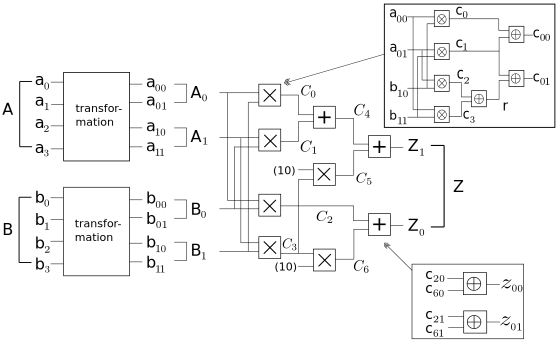
\includegraphics[width=.9\linewidth]{./figures/compMineSmall}
        \caption{$4$-bit composite multiplier designed over $\F_{(2^2)^2}$}\label{fig:comp4ex}
\end{figure}

Let $P(x) = x^4 + x^3 + 1$ and $P(\alpha)=0$. 
Representation of element $A \in \mathbb{F}_{(2^2)^2}$ is:
\begin{eqnarray}
A& = A_0 +A_1 \cdot \alpha
\end{eqnarray}
Representation of $A_0, A_1$ in $\mathbb{F}_{2^m}$ is:
\begin{eqnarray}
A_0=a_{00}+a_{01} \cdot \beta \nonumber \\
A_1=a_{10}+a_{11} \cdot \beta
\end{eqnarray}
where $a_{ij}\in \mathbb{F}_2$. From Eqn.(\ref{eqn:betaToAlpha}), $\beta=\alpha^5$
Now $A_0, A_1$ can be substituted into $A$ as follows:
\begin{eqnarray}
A&=&a_{00}+a_{01}\cdot \alpha^5+(a_{10}+a_{11}\cdot \alpha^5)\cdot \alpha
\end{eqnarray}
Since $P(x)=x^4+x^3+1$ with $P(\alpha)=0$,
\begin{equation}\label{a}
A \pmod {P(\alpha)}=a_{00}+a_{01}+a_{11}+(a_{01}+a_{10}+a_{11})\cdot \alpha+a_{1
1} \cdot \alpha^2+(a_{01}+a_{11})\cdot \alpha^3   
\end{equation}
The same element $A \in \mathbb{F}_{2^4}$ is represented as:
\begin{equation}\label{aa}
A=a_0+a_1\cdot \alpha+a_2\cdot \alpha^2+a_3\cdot \alpha^3 
\end{equation}

\item Since Eqns. (\ref{a}) and (\ref{aa}) represent the same element, we
  can match the coefficients of the the polynomials to obtain:
\begin{eqnarray}
a_0&=&a_{00}+a_{01}+a_{11} \nonumber \\
a_1&=&a_{01}+a_{10}+a_{11} \nonumber \\
a_2&=&a_{11} \nonumber \\
a_3&=&a_{01}+a_{11} \nonumber
\end{eqnarray}

This mapping can also be reversed and represented as a matrix $T^{-1}$:
\begin{equation}
\begin{bmatrix} a_{00}\\ a_{01} \\a_{10} \\ a_{11}\end{bmatrix}
=
\begin{bmatrix} 1 & 0 & 0 & 1\\ 0 & 0 & 1 & 1\\ 0 & 1 & 0 & 1\\ 0 & 0
  & 1 & 0 \end{bmatrix} 
\begin{bmatrix} a_0\\ a_1 \\a_2 \\ a_3\end{bmatrix}
\end{equation}
Thus, $A$ is represented in $\mathbb{F}_{(2^2)^2}$ as:
\begin{eqnarray}
A&=&A_0+A_1 \cdot \alpha \nonumber \\
A_0&=&a_{00}+a_{01} \cdot \alpha^5 \nonumber \\
A_1&=&a_{10}+a_{11} \cdot \alpha^5 \nonumber \\
a_{00}&=&a_0+a_3 \nonumber \\
a_{01}&=&a_2+a_3 \nonumber \\
a_{10}&=&a_1+a_3 \nonumber \\
a_{11}&=&a_2 \nonumber 
\end{eqnarray}
$B$ is similarly represented in $\mathbb{F}_{(2^2)^2}$.
\end{Example}

\subsection{Abstraction of Composite Field Multipliers}

The first step in abstracting the word-level polynomial representation of the composite field
multiplier is to abstract every internal $\F_{2^m}$ computational block. In the case of a $\F_{2^m}$
adder block ($\{Z_0,Z_1,C_4\}$ from Fig.(\ref{fig:comp4ex})), this abstraction is trivial, as the adder is just a bit-wise XOR computation. In the case
of a multiplier block ($\{C_0,C_1,C_2,C_3,C_5,C_6\}$ from Fig.(\ref{fig:comp4ex})), 
the abstraction approach presented in the previous chapter is directly 
applicable. Each abstraction can be computed independently, so these computations can be 
performed in parallel. This set of abstracted polynomials, $F$, generates the ideal $J$.

Once the word-level abstraction of each $\F_{2^m}$ sub-block is known, the final abstraction of the 
entire design can be computed using only word-level variables. Set a RATO ordering. Then
reduce the word level polynomial by $F+F_0$:
\begin{equation}
f_Z: Z_0+Z_1\alpha+\dots+Z_{n-1}\alpha^{n-1}+Z
\end{equation}
\begin{equation}
f_Z\xrightarrow{F+F_0}_+ r
\end{equation}
Here, $F$ is the set of word-level
polynomial abstractions from each $\F_{2^m}$ block and $F_0$ is the set of vanishing polynomials.
Every variable $X$, apart from the word-level inputs $A$ and $B$ and word-level output $Z$, is an element of
$\F_{2^m}$, so its corresponding vanishing polynomial is $X^{2^m}+X$. Computing the reduction
gives remainder $r$ containing the elements 
\begin{equation}
A_0,A_1,\dots,A_{n-1},B_0,B_1,\dots,B_{n-1},Z
\end{equation}
Similarly, the mapping from $\{A_0,\dots,A_{n-1}\}$ to $A$ now needs to be derived (along with
the mapping from $\{B_0,\dots,B_{n-1}\}$ to $B$). That is, the next step is to find 
\begin{eqnarray}
& &F_A=\{F_{A_0},F_{A_1},\dots,F_{A_{n-1}}\} \nonumber \\
\text{where }& &F_{A_i}=A_i+\Func_{A_i}(A)
\end{eqnarray}
$F_A$ is derived from the polynomial
\begin{equation}
A=A_0+A_1\alpha+\dots+A_{n-1}\alpha^{n-1}
\end{equation}
Compute $A^{2^m}$ as follows:
\begin{eqnarray}
A^{2^m}: & & (A_0+A_1\alpha+\dots+A_{n-1}\alpha^{n-1})^{2^m} \nonumber \\
&&=A_0^{2^m}+A_1^{2^m}\alpha^{2^m}+\dots+A_{n-1}^{2^m}\alpha^{2^m(n-1)} \nonumber \\
&&=A_0+A_1\alpha^{2^m}+\dots+A_{n-1}\alpha^{2^m(n-1)}
\end{eqnarray}
Here, the property is $A_i^{2^m}=A_i$ is exploited. Continually raise this result by $2^m$ 
to obtain $A^{2^{jm}}$ for all $0\leq j < n$. This gives a system of $n$ equations and $n$
unknowns $\{A_0,\dots,A_{n-1}\}$. As before, this system of equations can be represented
in matrix form, $\mathbf{A = M a}$, where 
$\mathbf{A}=\{A,A^{2^m},\dots,A^{2^{(n-1)m}}\}^T$, 
$\mathbf{M}$ is
a $n$ by $n$ matrix of coefficients $\in \Fkk$, and $\mathbf{a}=\{A_0,\dots,A_{n-1}\}^T$:

\begin{eqnarray}
\begin{bmatrix}
A \\ A^{2^m} \\ \vdots \\ A^{2^{(n-1)m}}
\end{bmatrix}  &=&
\begin{bmatrix}
1      &   \alpha          & \alpha^2         & \dots & \alpha^{n-1}\\
1      &   \alpha^{2^m}     & \alpha^{2\cdot2^m}    & \dots & \alpha^{(n-1)\cdot 2^m}\\
1      &   \alpha^{2^{2m}}   & \alpha^{2\cdot2^{2m}}    & \dots & \alpha^{(n-1)\cdot 2^{2m}}\\
\vdots & \vdots            & \vdots           & \cdot & \vdots \\
1      &   \alpha^{2^{(n-1)m}} & \alpha^{2\cdot2^{(n-1)m}} & \dots & \alpha^{(n-1)\cdot 2^{(n-1)m}}
\end{bmatrix}
\begin{bmatrix}
A_0 \\ A_1 \\ \vdots \\ A_{n-1}
\end{bmatrix} \label{eqn:matrixForm}
\end{eqnarray}

The matrix $\mathbf{M}$ is the Vandermonde matrix $V(\alpha,\alpha^{2^m},\dots,\alpha^{2^{(n-1)m}})$.
Since $\alpha$ is a primitive element, 
all elements $\alpha,\dots,\alpha^{2^{k-1}}$ are unique, where $k=m\cdot n$. Thus, 
all elements $\alpha,\alpha^{2^m},\dots,\alpha^{2^{(n-1)m}}$ are unique, so
$|\mathbf{M}| \neq 0$. Then, Cramer's rule can be applied to derive each $F_{A_i}$ as 
\begin{equation}
F_{A_i}=A_i+\frac{|\mathbf{M_i}|}{|\mathbf{M}|}
\end{equation}
where $\mathbf{M_i}$ is $\mathbf{M}$ with the $i$-th column replaced
by $\mathbf{A}$. Here, $|\mathbf{M}|$ is not guaranteed to be equal to $1$,  
%Rather, $|\mathbf{M}|$ is a non-zero element of $\F_{2^m}$ (proof in Appendix \ref{append:Fpk}),
so it must be computed. 
$F_B=\{F_{B_0},\dots,F_{B_{n-1}}\}$ is similarly derived.
Computing $r\xrightarrow{F_A,F_B,J_0}_+ r_w$ gives $r_w: Z+\Func(A,B)$ which is the 
canonical word-level polynomial abstraction of the composite field design.

\begin{Example}
Consider the composite field multiplier over $\F_{{2^2}^2}$ from Example \ref{ex:comp22}.
Abstracting every multiplier and adder over the base field $\F_{2^2}$ gives the following
polynomials:
\begin{eqnarray}
f_1: Z_0+C_6+C_2      & f_2: Z_1+C_5+C_4      & f_3: C_6+\alpha^5C_3 \nonumber \\
f_4: C_5+\alpha^5C_3  & f_5: C_4+C_1+C_0      & f_6: C_3+A_1\cdot B_1 \nonumber \\
f_7: C_2+A_0\cdot B_0 & f_8: C_1+A_1\cdot B_0 & f_9: C_0+A_0\cdot B_1 
\end{eqnarray}
Set the following RATO ordering:
\begin{eqnarray}
Z_0 > Z_1 > C_6 > C_5 > C_4 > C_3 > C_2 > C_1 > C_0 \nonumber \\
> A_0 > A_1 > B_0 > B_1 > Z > A > B
\end{eqnarray}
The vanishing polynomials are:
\begin{eqnarray}
f_{10}: Z_0^4+Z_0 & f_{11}: Z_1^4+Z_1 & f_{12}: C_6^4+C_6 \nonumber \\
f_{13}: C_5^4+C_5 & f_{14}: C_4^4+C_4 & f_{15}: C_3^4+C_3 \nonumber \\
f_{16}: C_2^4+C_2 & f_{17}: C_1^4+C_1 & f_{18}: C_0^4+C_0 \nonumber \\
f_{19}: A_0^4+A_0 & f_{20}: A_1^4+A_1 & f_{21}: B_0^4+B_0 \nonumber \\
f_{22}: B_1^4+B_1 & f_{23}: Z^{16}+Z  & f_{24}: A^{16}+A \nonumber \\
f_{25}: B^{16}+B
\end{eqnarray}
Then $F=f_1,\dots,f_9$ and 
$F_0=f_{10},\dots,f_{25}$.
Here, $f_Z: Z_0+Z_1\alpha+Z$. Computing $f_Z\xrightarrow{F,F_0}_+ r$ gives:
\begin{equation}
r= A_0\cdot B_0+\alpha A_0\cdot B_1+\alpha A_1\cdot B_0+\alpha^2A_1\cdot B_1+Z
\end{equation}

Next, $F_A=\{F_{A_0},F_{A_1}\}$ needs to be derived. Here, $A=A_0+A_1\alpha$ and $A^{4}=A_0+A_1\alpha^4$,
which gives
\begin{eqnarray}
\mathbf{M}=
\begin{bmatrix}
1 & \alpha \\
1 & \alpha^4
\end{bmatrix}; &
\mathbf{M_0}=
\begin{bmatrix}
A & \alpha \\
A^4 & \alpha^4
\end{bmatrix}; &
\mathbf{M_1}=
\begin{bmatrix}
1 & A \\
1 & A^4
\end{bmatrix}
\end{eqnarray}
After minimizing by the primitive polynomial $P(x)=x^4+x^3+1$, 
the determinants of these matrices are:
\begin{eqnarray}
|\mathbf{M}|=\alpha^3+\alpha+1; &
|\mathbf{M_0}|=\alpha A^4+(\alpha^3+1)A; &
|\mathbf{M_1}|=A^4+A
\end{eqnarray}
%Notice that $|\mathbf{M}|=\alpha^5=\beta\in\F_{2^2}$.%% NOTE: haven't figured out if this is always the case 
Now $F_{A_0}$ and $F_{A_1}$ are derived:
\begin{eqnarray}
F_{A_0} = &A_0+\frac{|\mathbf{M_0}|}{|\mathbf{M}|}& = A_0+(\alpha^3+\alpha^2+1)A^4+(\alpha^3+\alpha^2)A \\
F_{A_1} = &A_1+\frac{|\mathbf{M_1}|}{|\mathbf{M}|}& = A_1+(\alpha^3+\alpha)A^4+(\alpha^3+\alpha)A
\end{eqnarray}
Since $F_B=\{F_{B_0},F_{B_1}\}$ is derived from $B=B_0+B_1\alpha$, which is isomorphic to
$A=A_0+A_1\alpha$, then $F_B$ can be derived from $F_A$ by substituting corresponding
variables.
\begin{eqnarray}
F_{B_0}& = &B_0+(\alpha^3+\alpha^2+1)B^4+(\alpha^3+\alpha^2)B \\
F_{B_1}& = &B_1+(\alpha^3+\alpha)B^4+(\alpha^3+\alpha)B
\end{eqnarray}
Finally, computing $r\xrightarrow{F_A,F_B,F_0}_+ r_w$ gives the word-level abstraction of
the circuit.
\begin{equation}
r_w: Z+A\cdot B
\end{equation}


\end{Example}

\section{Conclusion}

This chapter described how to generalize the abstraction approach to any arbitrary
combinational circuit. This method works best when the derived operand-width $k$, from the $LCM$ of the 
word-lengths of all inputs and output, is not very large, for instance, when the output size is a 
multiple of the input sizes. When all word-sizes are relatively prime,
$k$ is a product of all sizes, which can make the analysis overly bulky.

An abstraction technique for exploiting the hierarchy of composite field multiplier circuits over
$\F_{(2^m)^n} $
was also examined. The approach abstracts all internal multipliers and adders over $\F_{2^m}$ in 
parallel and uses these abstractions to compute the final abstraction completely over
word-level variables. Experimental results for abstractions of composite field multipliers using a
custom-built tool is presented in the next chapter.
